\documentclass[a4paper]{article}
\linespread{1.6}
\usepackage{geometry}
\usepackage{setspace}
\usepackage{amsmath}
\usepackage{amssymb}
\usepackage{enumerate}
\usepackage[pdftex]{graphicx}
\usepackage{float}
\usepackage{subfigure}
\usepackage{listings}
\geometry{left=1.5cm,right=1.5cm,top=2.5cm,bottom=2.5cm}

\begin{document}
\begin{spacing}{2.0}
\begin{flushleft}\begin{huge}EEE5502 Foundations of Digital Signal Processing   Code 5\end{huge}\end{flushleft}
\begin{flushright}\begin{Large} Hudanyun Sheng \end{Large}\end{flushright}

\Large\textbf{ Question \#1}:  \\
\normalsize
I spent 8 hours.\\

\Large\textbf{Question \#2}:  
\normalsize
\begin{enumerate}[(a)]
\item $\omega[n] = \displaystyle\frac{4\pi n}{10000} =  \displaystyle\frac{\pi n}{2500} $

\item $\omega[0] = 0\pi$, $\omega[2500] = \pi$.

\item The length-2501 signal $x[n]$ is shown below:
\begin{figure} [H]
\centering
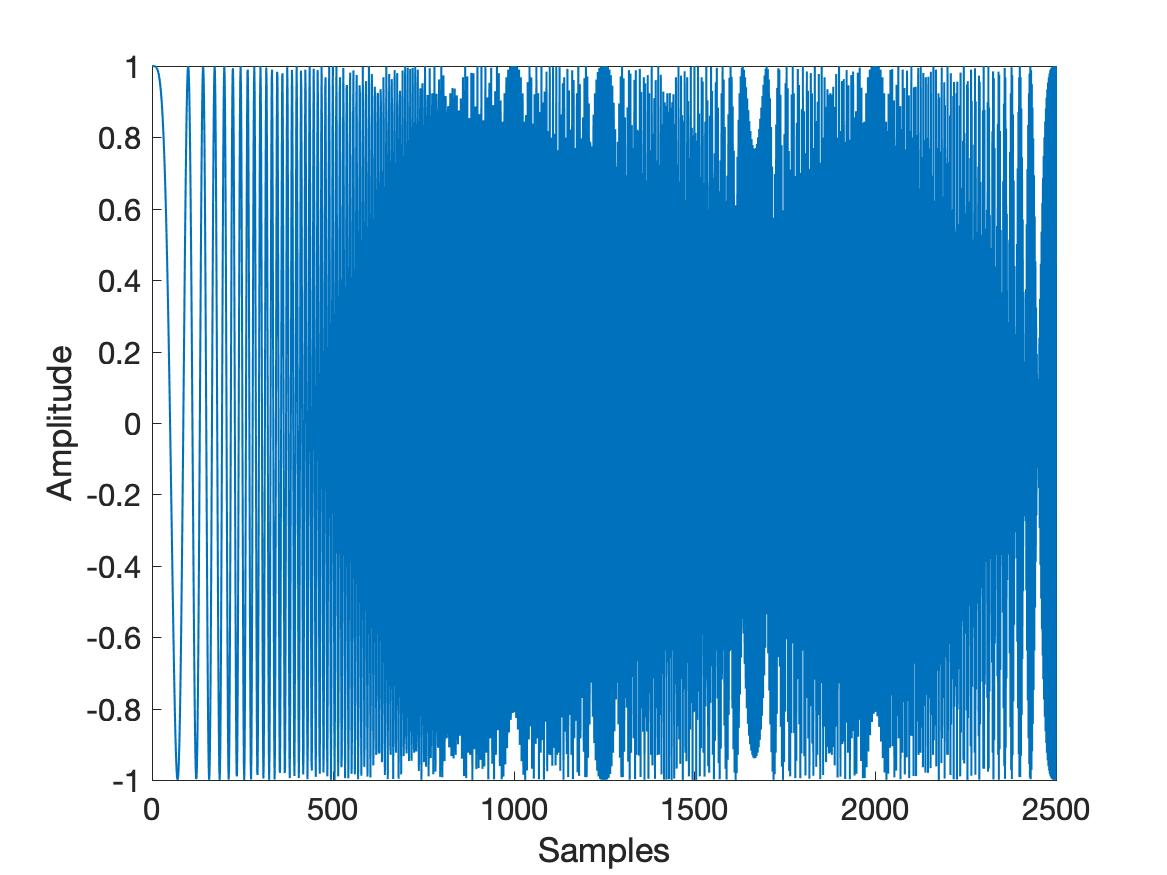
\includegraphics[width=3in]{Q2partc.jpg}
\caption{The length-2501 signal $x[n]$}
\label{fig:graph}
\end{figure}

\item The magnitude plot of the DFT of signal $x[n]$ is shown below:
\begin{figure}[H]
\centering
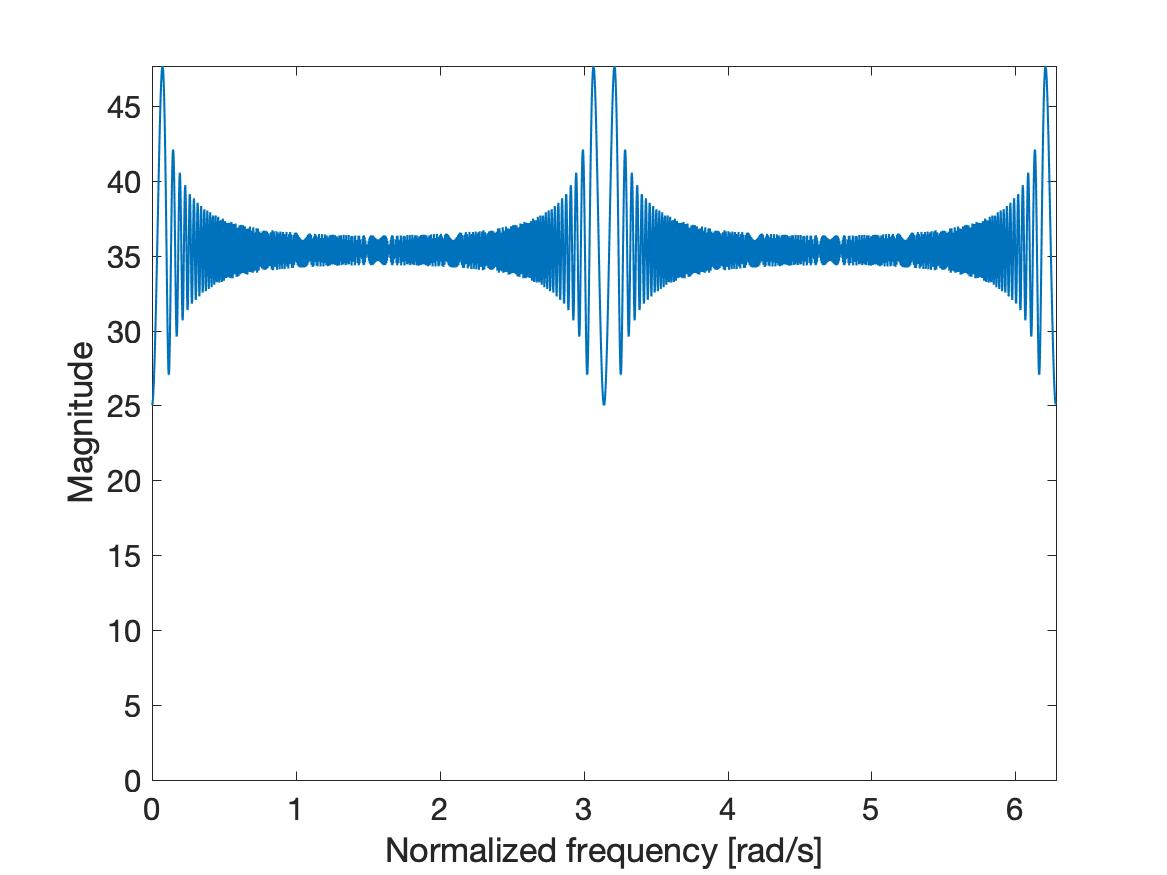
\includegraphics[width=3in]{Q2partd.jpg}
\caption{The magnitude of the DFT of signal $x[n]$}
\end{figure}

\item The phase plot of the DFT of signal $x[n]$ is shown below:
\begin{figure}[H]
\centering
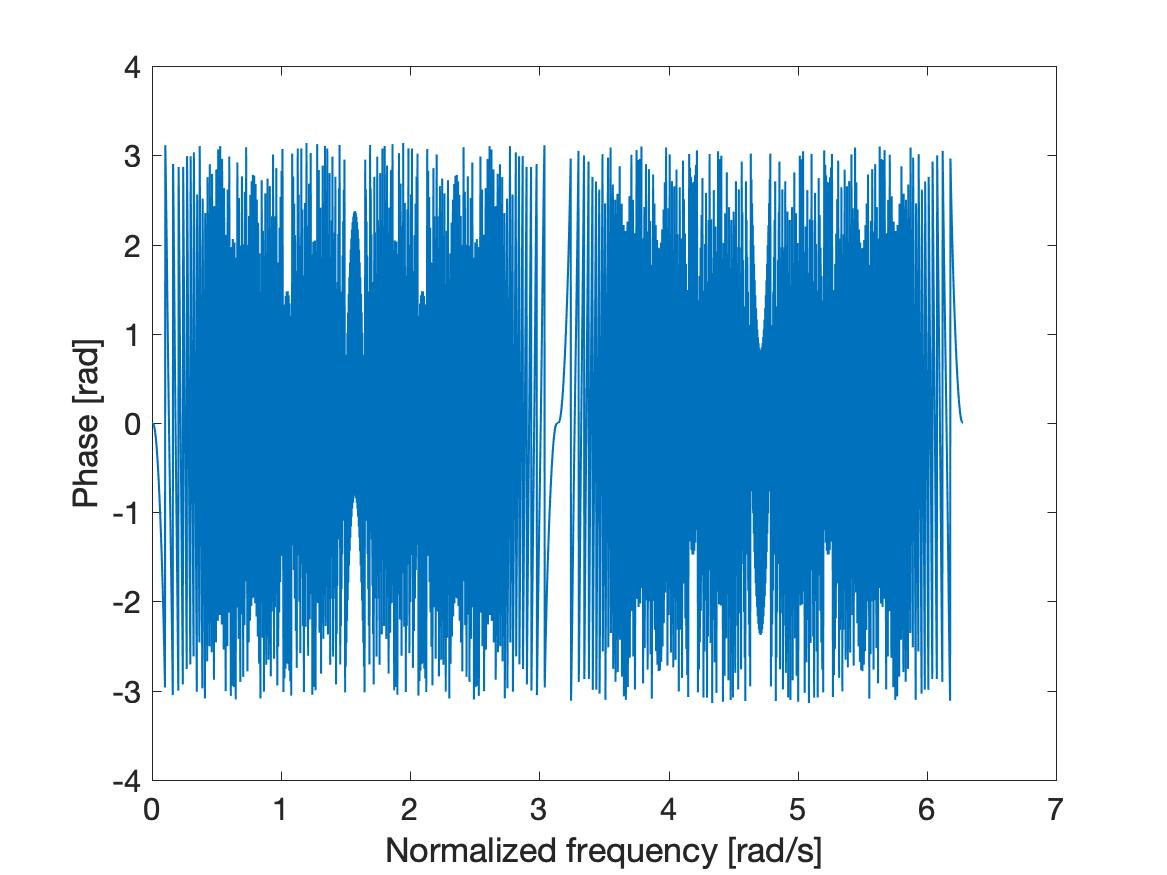
\includegraphics[width=3in]{Q2parte.jpg}
\caption{The phase of the DFT of signal $x[n]$}
\end{figure}

\item Delta function has a similar magnitude response in frequency domain. They are significantly different in time is because the function in this problem has limit in time. Thus unlike the Delta function, it is unable to pertain that much information.
\end{enumerate}

\Large\textbf{Question \#3}:
\normalsize
\begin{enumerate}[(a)]
\item All code for this question is attached as a .m file.

\item The plots of short-time Fourier transform for 8 different values of W are shown below:
\begin{figure}[H]
\centering
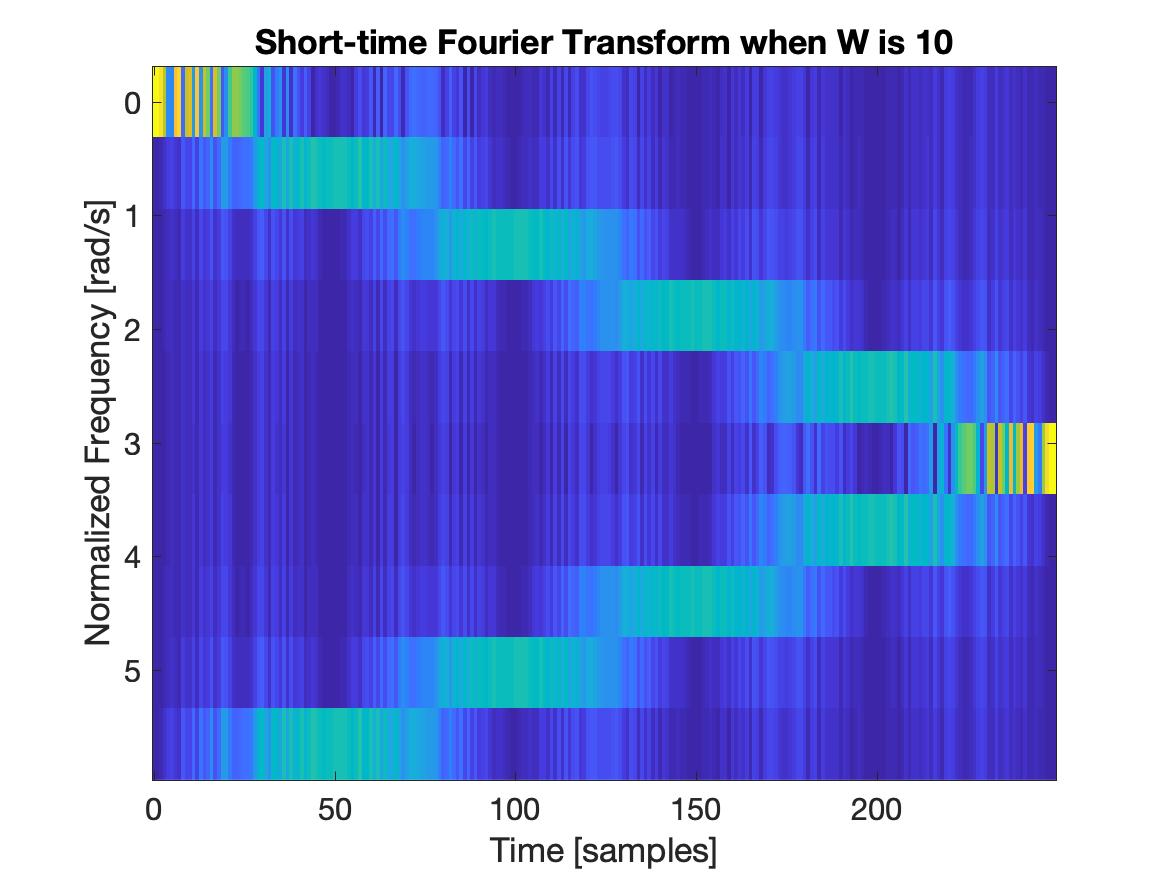
\includegraphics[width=2.5in]{Q3W10.jpg}
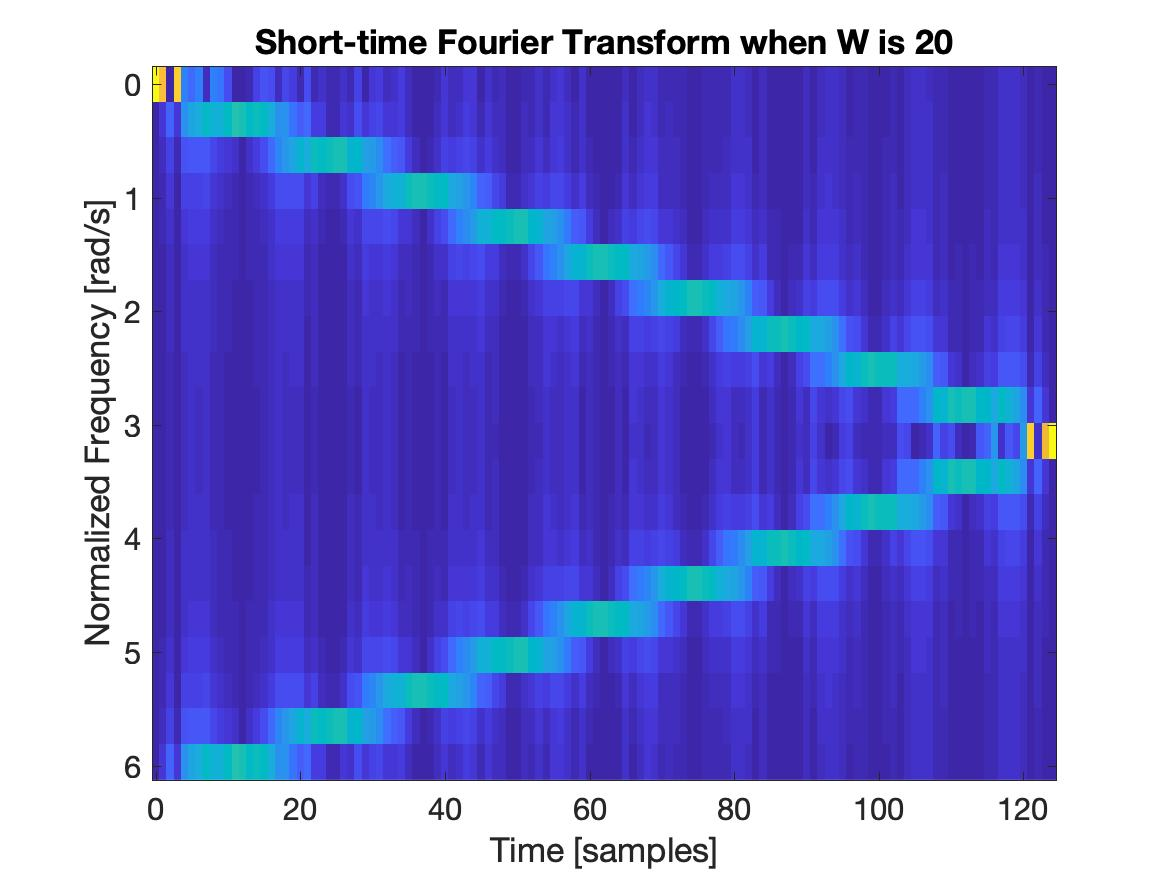
\includegraphics[width=2.5in]{Q3W20.jpg}
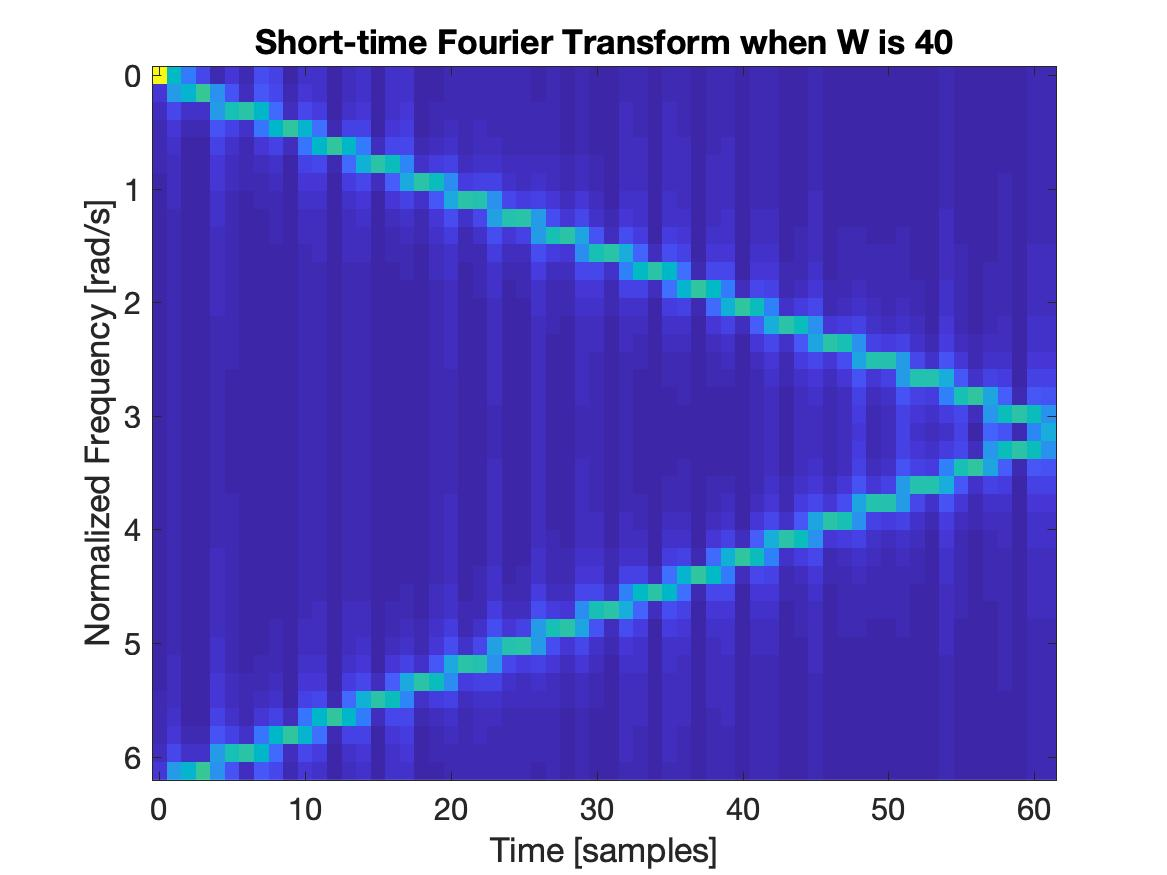
\includegraphics[width=2.5in]{Q3W40.jpg}
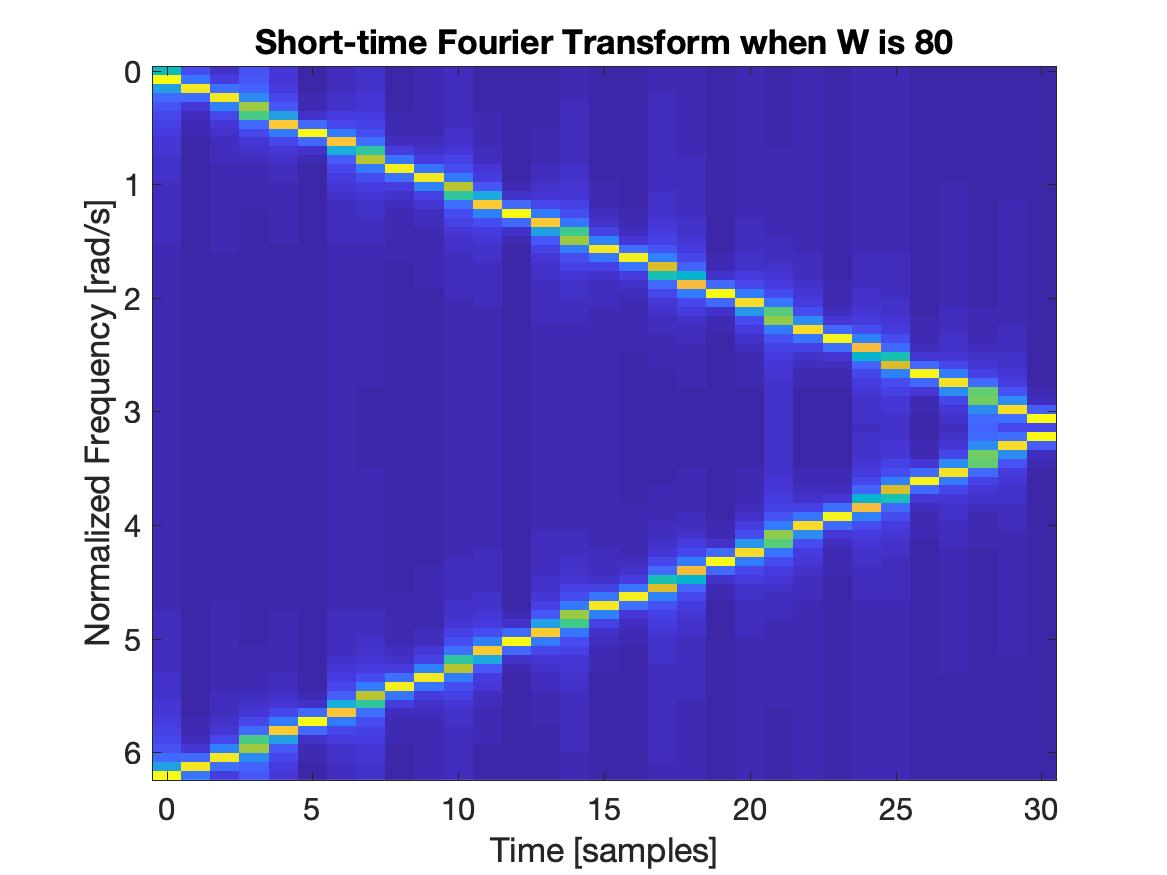
\includegraphics[width=2.5in]{Q3W80.jpg}
\caption{The plots of short-time Fourier transform when W is 10 (top left), 20 (top right), 40 (bottom left) and 80(bottom right) respectively.}
\end{figure}

\begin{figure}[H]
\centering
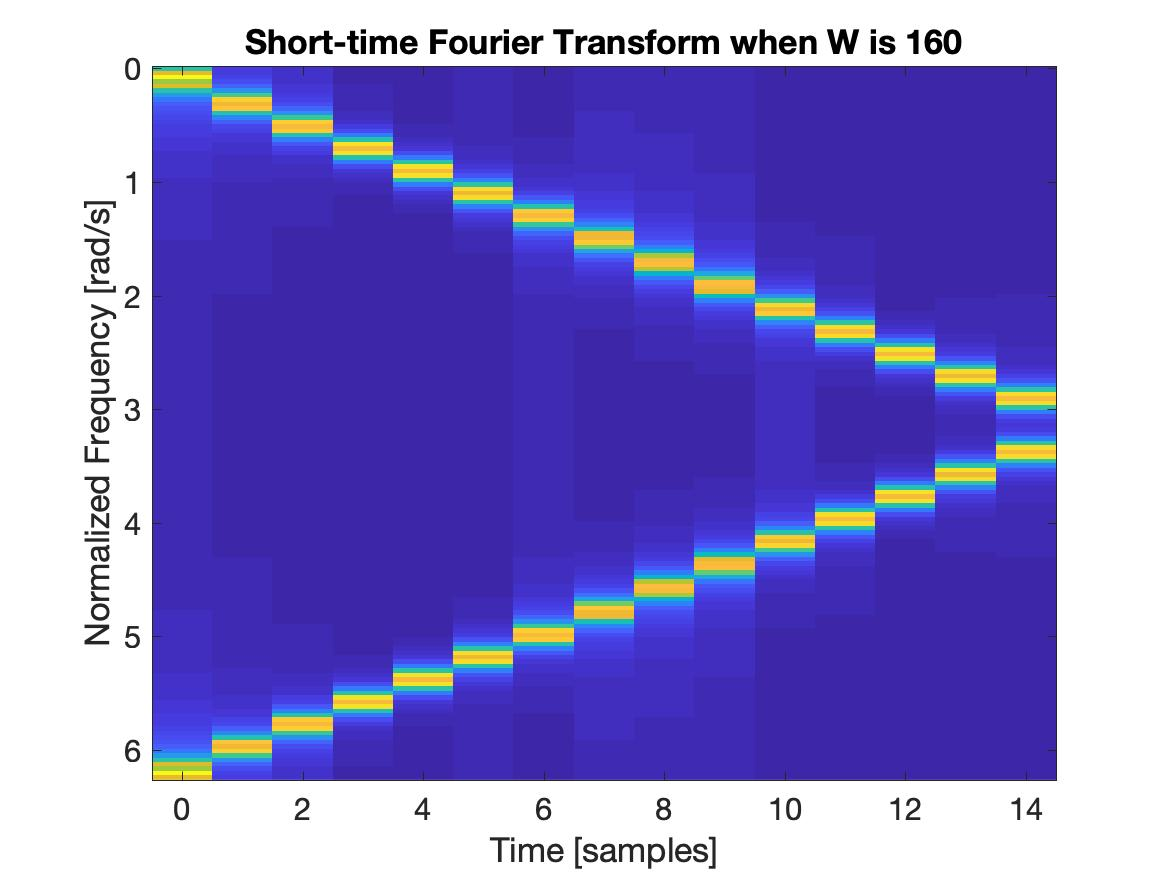
\includegraphics[width=2.5in]{Q3W160.jpg}
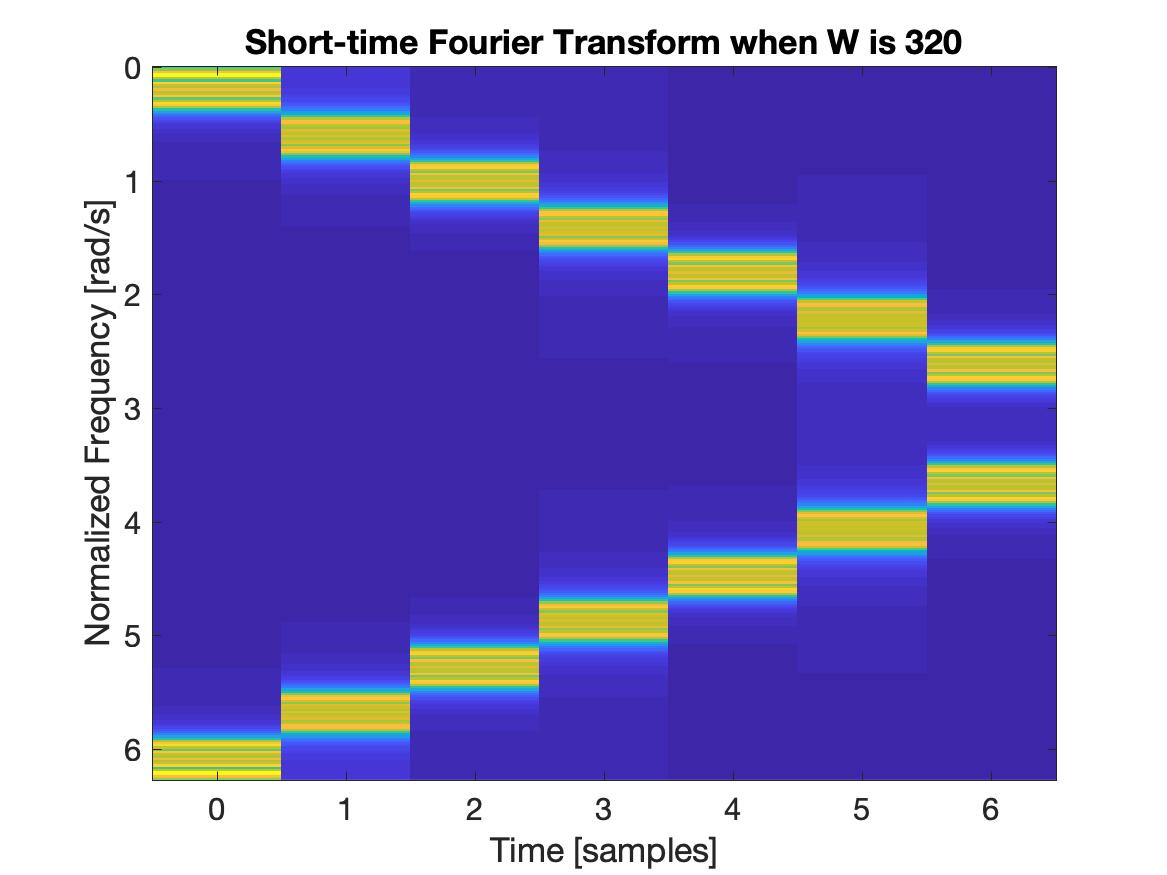
\includegraphics[width=2.5in]{Q3W320.jpg}
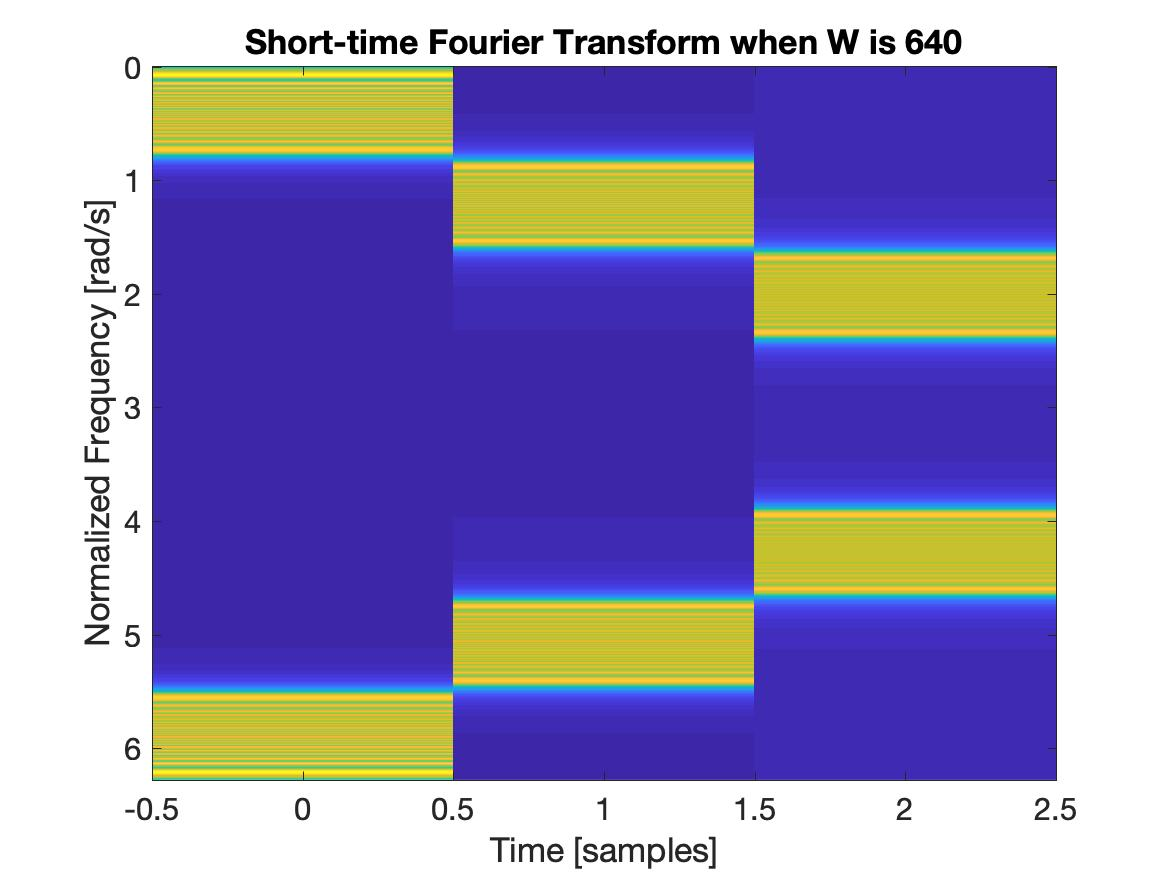
\includegraphics[width=2.5in]{Q3W640.jpg}
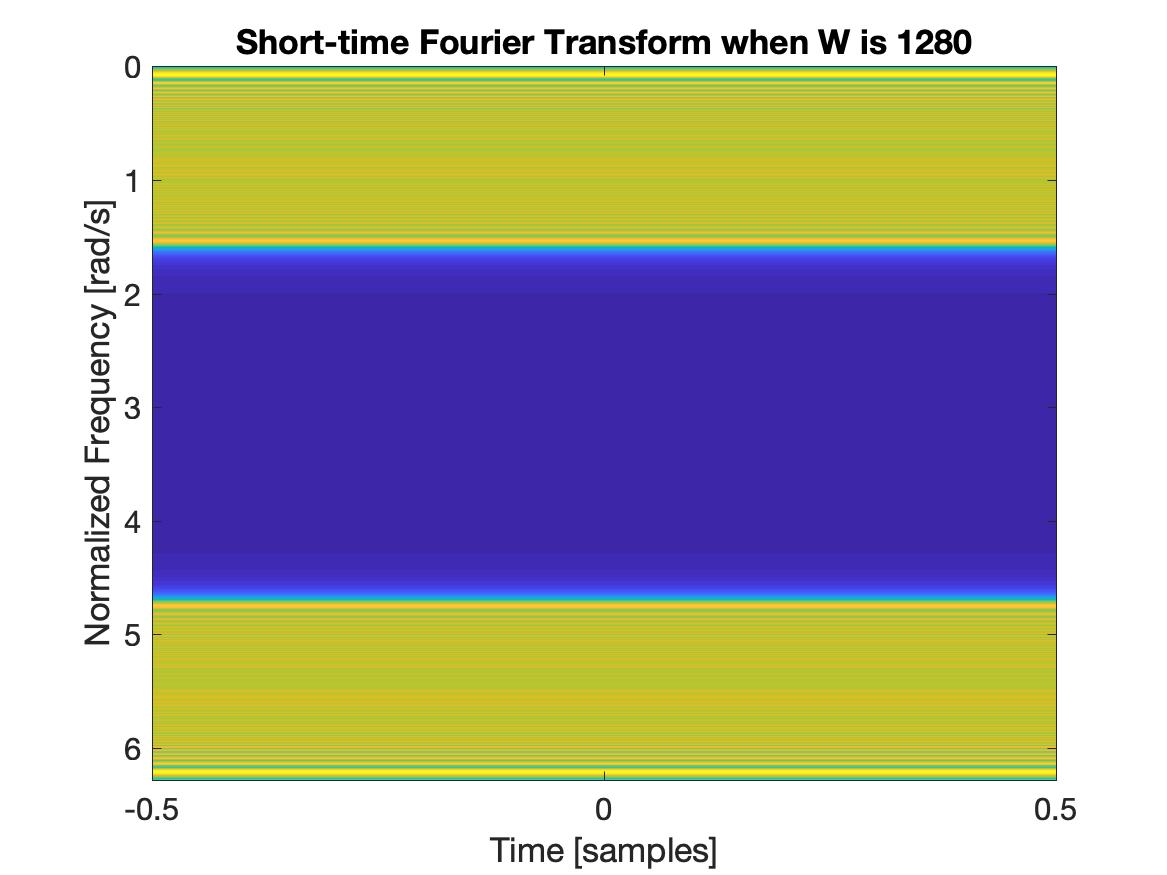
\includegraphics[width=2.5in]{Q3W1280.jpg}
\caption{The plots of short-time Fourier transform when W is 160 (top left), 320 (top right), 640 (bottom left) and 1280(bottom right) respectively.}
\end{figure}

\item I think the value of W being 80 best illustrates the chirp signal.

\end{enumerate}

\Large\textbf{Question \#4}:
\normalsize
\begin{enumerate}[(a)]
\item The short-time Fourier transform of Rudenko music x is shown below:
\begin{figure}[H]
\centering
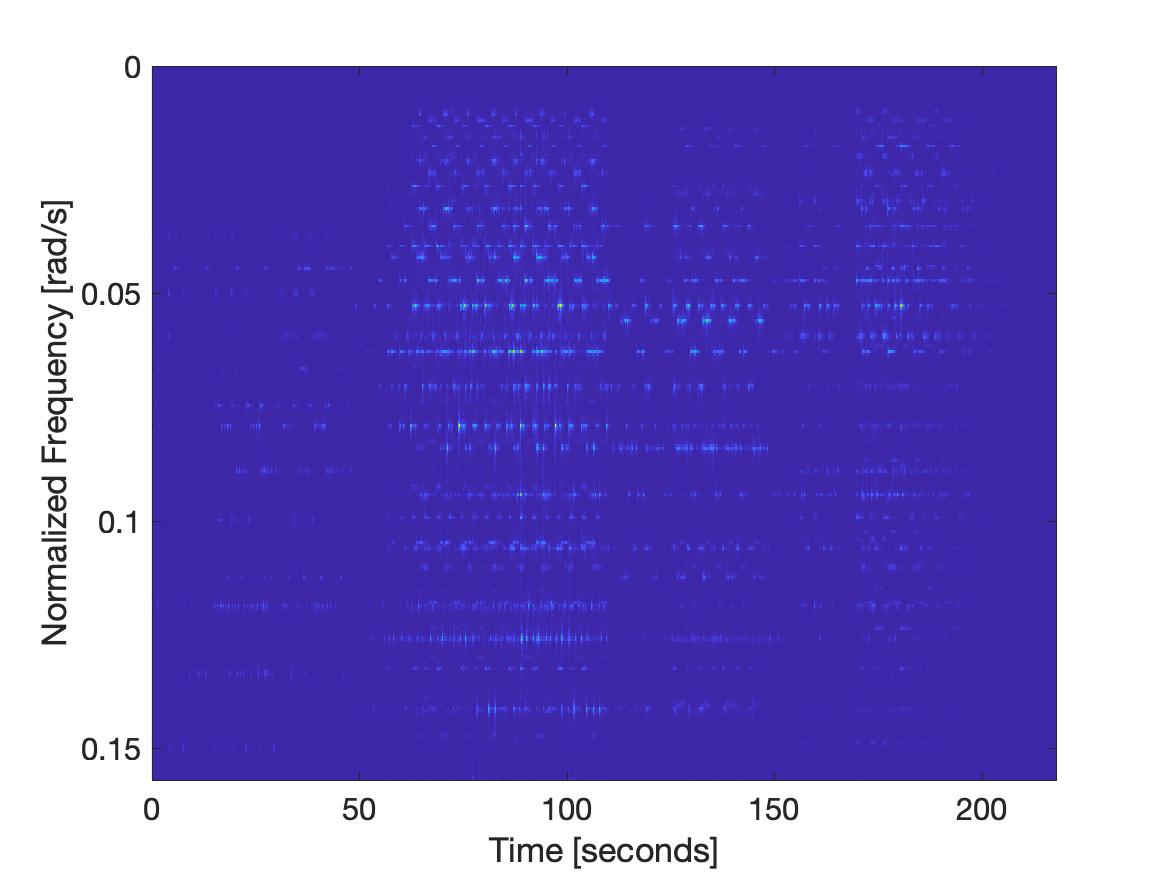
\includegraphics[width=4in]{Q4parta.jpg}
\caption{The plots of short-time Fourier transform of Rudenko music x.}
\end{figure}

\item The short-time Fourier transform of Rudenko music x with normalized frequency is shown below:
\begin{figure}[H]
\centering
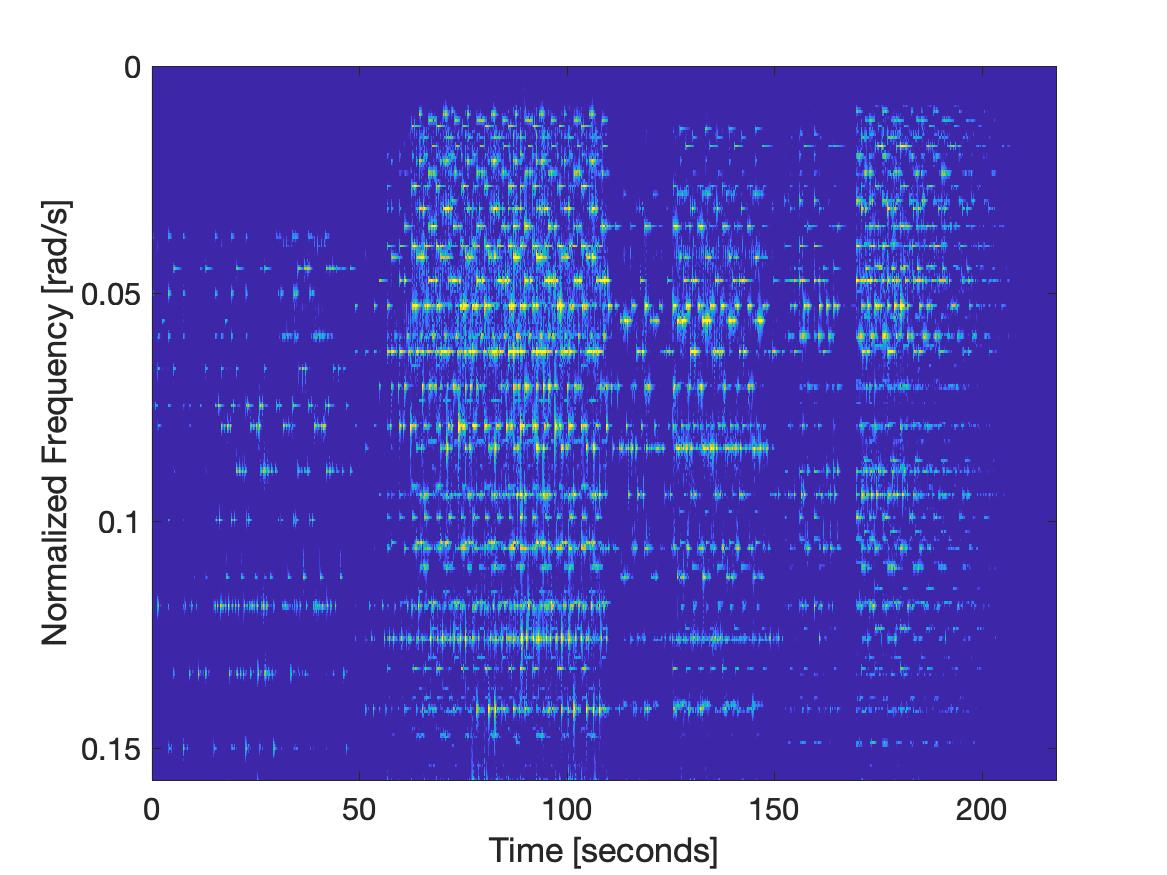
\includegraphics[width=4in]{Q4partb.jpg}
\caption{The plot of short-time Fourier transform of Rudenko music x with normalized data.}
\end{figure}

\item The short-time Fourier transform of the result of convolving Rudenko music with an average filter is shown below:
\begin{figure}[H]
\centering
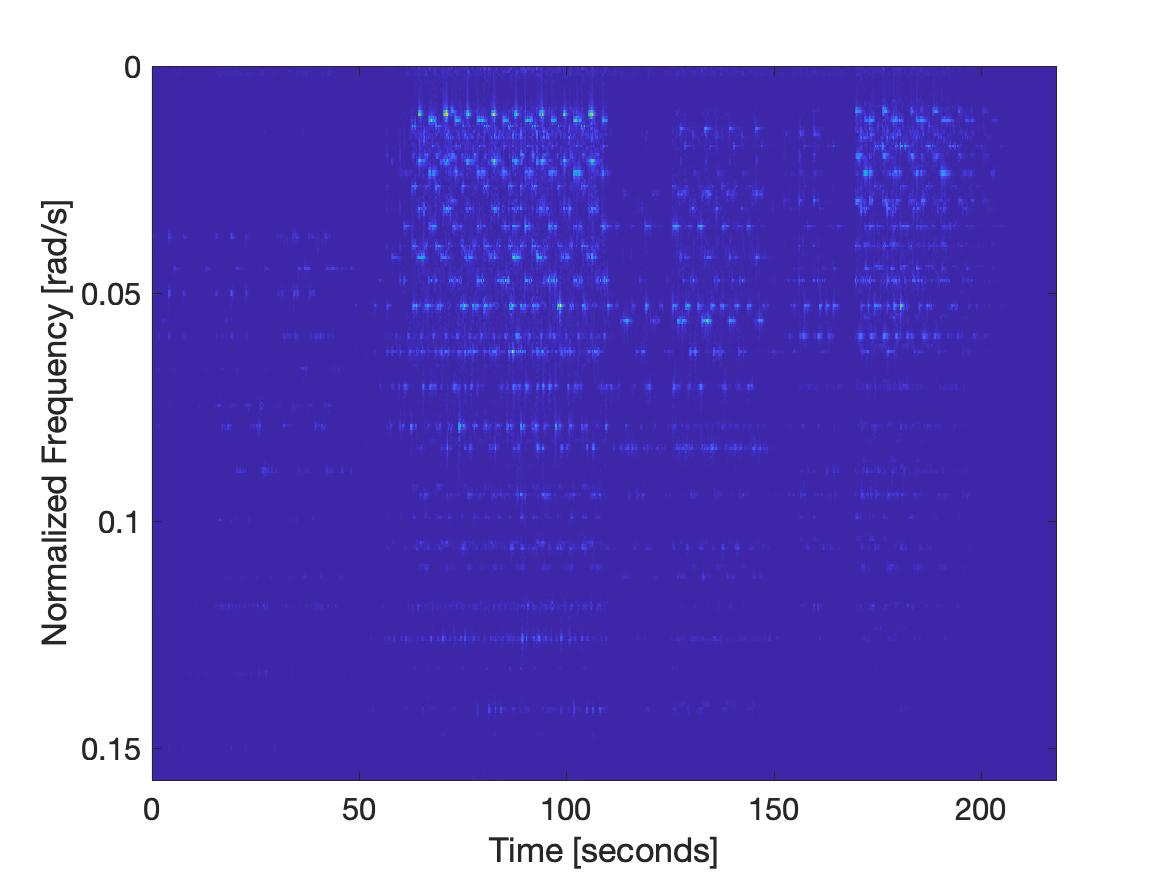
\includegraphics[width=3in]{Q4partc1.jpg}
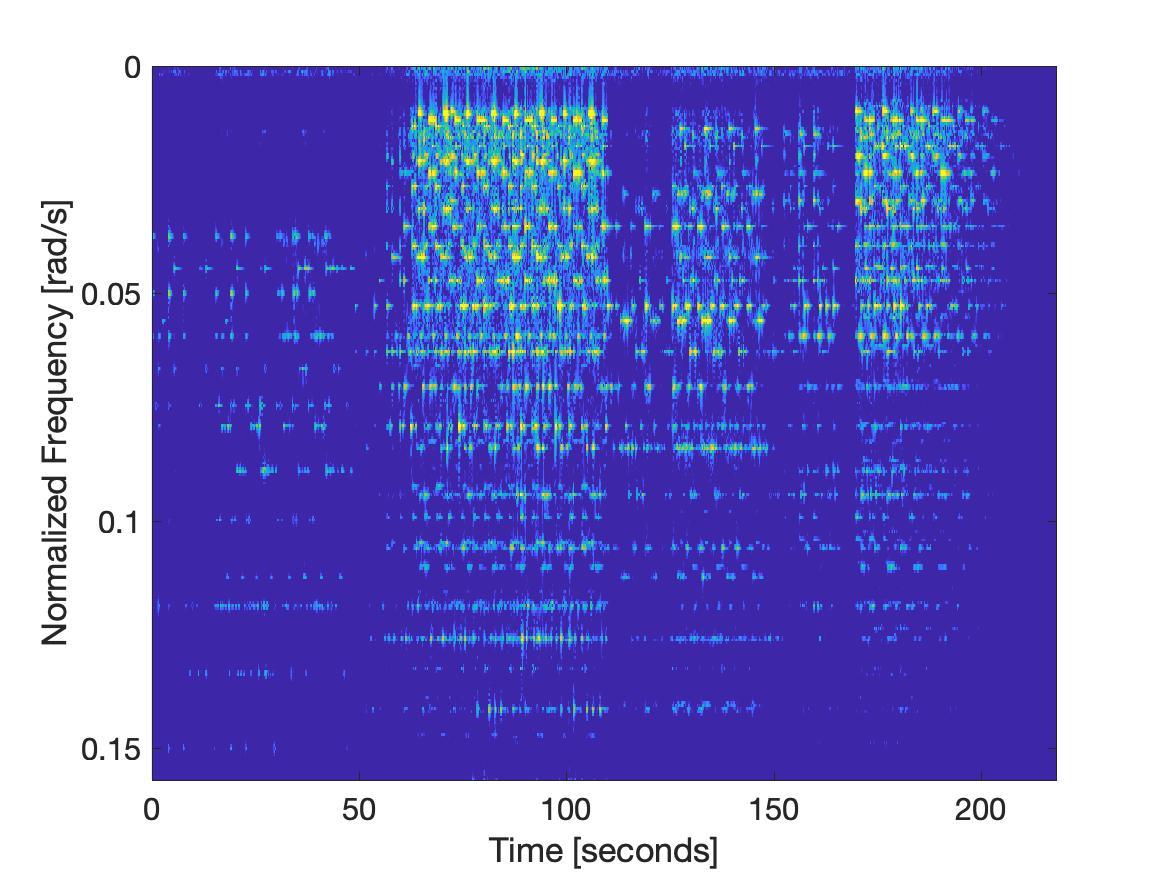
\includegraphics[width=3in]{Q4partc2.jpg}
\caption{The plot of short-time Fourier transform of the result of convolving Rudenko music with an average filter(left), with normalized data(right)}
\end{figure}

\item With data being normalized so that the maximum value is 1 would make the plots easier to visualize. Convolving the original data with a mean filter would decrease the strength of the signal in time domain, which, result in having to enlarge the signal to be able to hear. What is more, convolving with a mean filter would result in more components in frequency domain, and some increase of response at some frequency, as can be seen in plots. Correspondingly in time domain, we hear that the music changes some frequency.
\end{enumerate}


\end{spacing}
\end{document}